\usetikzlibrary{arrows.meta,decorations.pathmorphing}

\begin{frame}{kill() not always immediate}
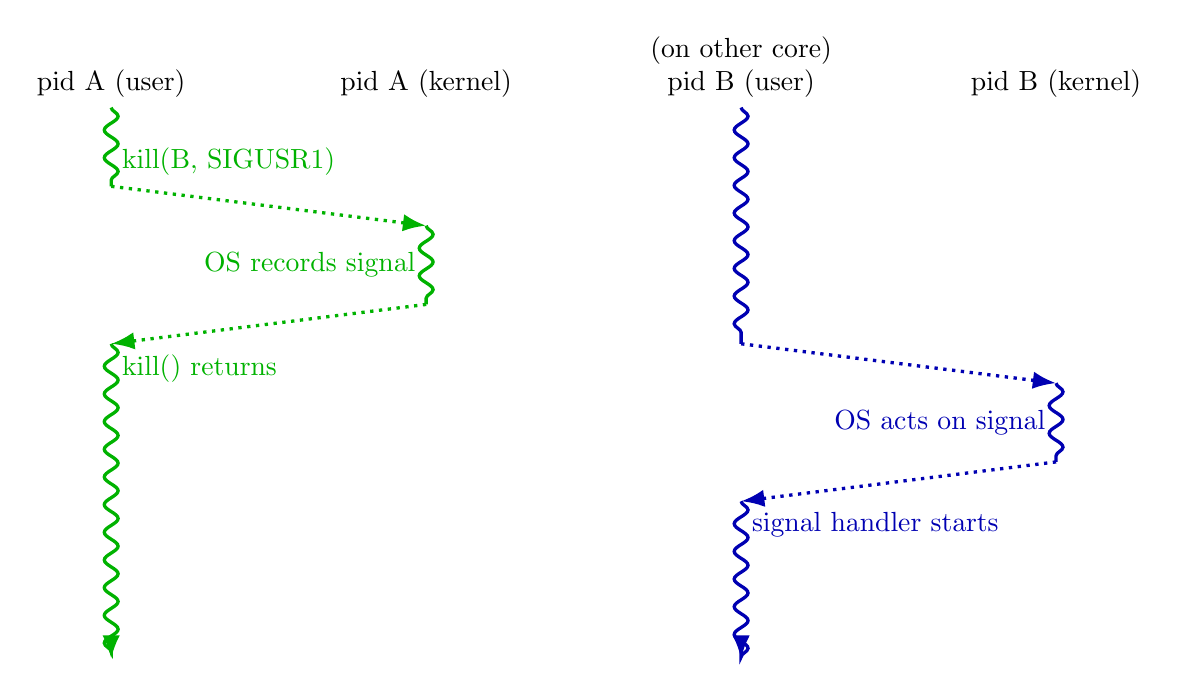
\begin{tikzpicture}
\tikzset{
    snake/.style={very thick,decorate,decoration={snake}},
    mode/.style={very thick,->,dotted},
    >=Latex,
    process A/.style={green!70!black},
    process B/.style={blue!70!black},
}
\draw[snake,process A] (0, 0) coordinate (A start) -- ++(0, -1)
    coordinate (A kill)
    node[above right] {kill(B, SIGUSR1)};
\node[anchor=south] at (A start) {pid A (user)};
\node[anchor=south] at ([xshift=4cm]A start) {pid A (kernel)};
\draw[mode,process A] (A kill) -- ++(4, -.5) coordinate (A kill sys);
\draw[snake,process A] (A kill sys) -- ++ (0, -1) coordinate (A ret kill sys)
    node[midway, left] {OS records signal};
\draw[mode,process A] (A ret kill sys) -- ++(-4, -.5) coordinate (A restart);
\draw[snake,process A,->] (A restart) -- ++(0, -4)
    node[pos=0,below right] {kill() returns};

\draw[snake,process B] (8, 0) coordinate (B start) -- ++(0, -3) coordinate (B intr);
\node[anchor=south,align=center] at (B start) {(on other core) \\ pid B (user)};
\node[anchor=south,align=center] at ([xshift=4cm]B start) {pid B (kernel)};
\draw[mode,process B] (B intr) -- ++(4, -.5) coordinate (B intr kern);
\draw[snake,process B] (B intr kern) -- ++ (0, -1) coordinate (A ret kill sys)
    node[midway, left] {OS acts on signal};
\draw[mode,process B] (A ret kill sys) -- ++(-4, -.5) coordinate (A restart);
\draw[snake,process B,->] (A restart) -- ++(0, -2)
    node[pos=0,below right] {signal handler starts};
\end{tikzpicture}
\end{frame}
